\label{ap:ap13}
\chapter{Frameworks de IA}
\section*{\textbf{A - ENUNCIADO}}

\subsection*{\textbf{1 Classificação (RNA)}}


Implementar o exemplo de Classificação usando a base de dados Fashion MNIST e a arquitetura RNA vista na aula
\textbf{FRA - Aula 10 - 2.4 Resolução de exercício de RNA - Classificação}. Além disso, fazer uma breve explicação dos
seguintes resultados: 

\begin{itemize}[series=listWWNumxiv,label={}-]
\item Gráficos de perda e de acurácia;
\item \ Imagem gerada na seção “\textbf{\textcolor[HTML]{2F5496}{Mostrar algumas classificações erradas”}}, apresentada
na aula prática.
\end{itemize}
Informações:

\begin{itemize}[series=listWWNumxiii,label=${\bullet}$]
\item \textbf{Base de dados: }Fashion MNIST Dataset 
\item \textbf{Descrição}: Um dataset de imagens de roupas, onde o objetivo é classificar o tipo de vestuário. É
semelhante ao famoso dataset MNIST, mas com peças de vestuário em vez de dígitos.
\item \textbf{Tamanho}: 70.000 amostras, 784 features (28x28 pixels).
\end{itemize}
\begin{itemize}[series=listWWNumxvi,label=${\bullet}$]
\item \textbf{Importação do dataset}: Copiar código abaixo.
\end{itemize}

\foreignlanguage{english}{\textcolor[HTML]{188038}{data = tf.keras.datasets.fashion\_mnist }}

\foreignlanguage{english}{\textcolor[HTML]{188038}{(x\_train, y\_train), (x\_test, y\_test) =
fashion\_mnist.load\_data()}}


\subsection*{\textbf{2 Regressão (RNA)}}


Implementar o exemplo de Classificação usando a base de dados Wine Dataset e a arquitetura RNA vista na aula \textbf{FRA
- Aula 12 - 2.5 Resolução de exercício de RNA - Regressão}. Além disso, fazer uma breve explicação dos seguintes
resultados: 

\begin{itemize}
\item Gráficos de avaliação do modelo (loss);
\item Métricas de avaliação do modelo (pelo menos uma entre MAE, MSE, R²).
\end{itemize}
Informações:

\begin{itemize}
\item \textbf{Base de dados: }Wine Quality
\item \textbf{Descrição}: O objetivo deste dataset prever a qualidade dos vinhos com base em suas características
químicas. A variável target (y) neste exemplo será o score de qualidade do vinho, que varia de 0 (pior qualidade) a 10
(melhor qualidade)
\item \textbf{Tamanho}: 1599 amostras, 12 features.
\end{itemize}
\begin{itemize}
\item \textbf{Importação}: Copiar código abaixo.
\end{itemize}

\foreignlanguage{english}{\textcolor[HTML]{188038}{url =
{\textquotedbl}https://archive.ics.uci.edu/ml/machine-learning-databases/wine-quality/winequality-red.csv{\textquotedbl}}}

\textcolor[HTML]{188038}{data = pd.read\_csv(url, delimiter=';')}


\textcolor[HTML]{188038}{Dica 1. Para facilitar o trabalho, renomeie o nome das colunas para português, dessa forma:}


\textcolor[HTML]{188038}{data.columns = [}

\textcolor[HTML]{188038}{\ \ \ \ {}'acidez\_fixa', \ \ \ \ \ \ \ \ \ \ \ \# fixed acidity}

\textcolor[HTML]{188038}{\ \ \ \ {}'acidez\_volatil', \ \ \ \ \ \ \ \ \# volatile acidity}

\textcolor[HTML]{188038}{\ \ \ \ {}'acido\_citrico', \ \ \ \ \ \ \ \ \ \# citric acid}

\textcolor[HTML]{188038}{\ \ \ \ {}'acucar\_residual', \ \ \ \ \ \ \ \# residual sugar}

\textcolor[HTML]{188038}{\ \ \ \ {}'cloretos', \ \ \ \ \ \ \ \ \ \ \ \ \ \ \# chlorides}

\textcolor[HTML]{188038}{\ \ \ \ {}'dioxido\_de\_enxofre\_livre', \# free sulfur dioxide}

\textcolor[HTML]{188038}{\ \ \ \ {}'dioxido\_de\_enxofre\_total', \# total sulfur dioxide}

\textcolor[HTML]{188038}{\ \ \ \ {}'densidade', \ \ \ \ \ \ \ \ \ \ \ \ \ \# density}

\textcolor[HTML]{188038}{\ \ \ \ {}'pH', \ \ \ \ \ \ \ \ \ \ \ \ \ \ \ \ \ \ \ \ \# pH}

\textcolor[HTML]{188038}{\ \ \ \ {}'sulfatos', \ \ \ \ \ \ \ \ \ \ \ \ \ \ \# sulphates}

\textcolor[HTML]{188038}{\ \ \ \ {}'alcool', \ \ \ \ \ \ \ \ \ \ \ \ \ \ \ \ \# alcohol}

\textcolor[HTML]{188038}{\ \ \ \ {}'score\_qualidade\_vinho' \ \ \ \ \ \ \ \ \ \ \ \ \ \ \# quality}

\textcolor[HTML]{188038}{]}


\textcolor[HTML]{188038}{Dica 2. Separe os dados (x e y) de tal forma que a última coluna (índice -1), chamada
score\_qualidade\_vinho, seja a variável target (y)}


\subsection*{\textbf{3 Sistemas de Recomendação}}


Implementar o exemplo de Sistemas de Recomendação usando a base de dados Base\_livos.csv e a arquitetura vista na aula
\textbf{FRA - Aula 22 - 4.3 Resolução do Exercício de Sistemas de Recomendação}. Além disso, fazer uma breve explicação
dos seguintes resultados:

\begin{itemize}[series=listWWNumxv,label=${\bullet}$]
\item Gráficos de avaliação do modelo (loss);
\item Exemplo de recomendação de livro para determinado Usuário.
\end{itemize}
Informações:

\begin{itemize}[series=listWWNumxvii,label=${\bullet}$]
\item \textbf{Base de dados: }Base\_livros.csv
\item \textbf{Descrição}: Esse conjunto de dados contém informações sobre avaliações de livros (Notas), nomes de livros
(Titulo), ISBN e identificação do usuário (ID\_usuario)
\item \textbf{Importação: }Base de dados disponível no Moodle (UFPR Virtual), chamada Base\_livros (formato .csv).
\end{itemize}

\subsection*{\textbf{4 Deepdream}}


Implementar o exemplo de implementação mínima de Deepdream usando uma imagem de um felino \ {}- retirada do site
Wikipedia - e a arquitetura Deepdream vista na aula \textbf{FRA - Aula 23 - Prática Deepdream}. Além disso, fazer uma
breve explicação dos seguintes resultados: 

\begin{itemize}
\item Imagem onírica obtida por \textit{Main Loop};
\item Imagem onírica obtida ao levar o modelo até uma oitava;
\item Diferenças entre imagens oníricas obtidas com \ \textit{Main Loop }e levando o modelo até a oitava.
\end{itemize}
Informações:

\begin{itemize}[resume*=listWWNumxiii]
\item \textbf{Base de dados: }\url{https://commons.wikimedia.org/wiki/File:Felis_catus-cat_on_snow.jpg}
\end{itemize}
\begin{itemize}
\item \textbf{Importação da imagem}: Copiar código abaixo.
\end{itemize}

\foreignlanguage{english}{\textcolor[HTML]{188038}{url =
{\textquotedbl}}}\url{https://commons.wikimedia.org/wiki/Special:FilePath/Felis_catus-cat_on_snow.jpg}\foreignlanguage{english}{\textcolor[HTML]{188038}{{\textquotedbl}}}


\textcolor[HTML]{188038}{Dica: Para exibir a imagem utilizando display (display.html) use o \\link
https://commons.wikimedia.org/wiki/File:Felis\_catus-cat\_on\_snow.jpg}


%%%%%%%%%%%%%%%%%%%%%%%%%%%%%%%%%%%%%%%%%%%%%%%%%%%%%%%%%%%%%%%%%%%%%%%%%%%%%%%%%%%%%%%%%%%%%
\section*{\textbf{B - RESOLUÇÃO}}

\subsection*{\textbf{1 Classificação (RNA)}}
\subsubsection*{Importação das bibliotecas}
\begin{lstlisting}[language=Python, style=input]
import tensorflow as tf
import matplotlib.pyplot as plt
import numpy as np
from mlxtend.plotting import plot_confusion_matrix
from sklearn.metrics import confusion_matrix
\end{lstlisting}
\subsubsection*{Importação dos dados}
\begin{lstlisting}[language=Python, style=input]
fashion_mnist = tf.keras.datasets.fashion_mnist
(x_train, y_train), (x_test, y_test) = fashion_mnist.load_data()
print("x_train.shape: ", x_train.shape)
print("y_train.shape: ", y_train.shape)
print("x_test.shape: ", y_test.shape)
print("y_test.shape: ", y_test.shape)
\end{lstlisting}
\begin{lstlisting}[language=, style=output]
x_train.shape:  (60000, 28, 28)
y_train.shape:  (60000,)
x_test.shape:  (10000,)
y_test.shape:  (10000,)
\end{lstlisting}
\subsubsection*{Pré-processamento}
\begin{lstlisting}[language=Python, style=input]
x_train, x_test = x_train/255.0, x_test/255.0
\end{lstlisting}
\subsubsection*{Criação do modelo}
\begin{lstlisting}[language=Python, style=input]
i = tf.keras.layers.Input(shape=(28, 28))
x = tf.keras.layers.Flatten()(i)
x = tf.keras.layers.Dense(128, activation="relu")(x)
x = tf.keras.layers.Dropout(0.2)(x)
x = tf.keras.layers.Dense(10, activation="softmax")(x)

model = tf.keras.models.Model(i, x)
\end{lstlisting}
\subsubsection*{Compilação e treinamento do modelo}
\begin{lstlisting}[language=Python, style=input]
model.compile(optimizer='adam',
              loss='sparse_categorical_crossentropy',
              metrics=['accuracy'])

r = model.fit(x_train,
              y_train,
              validation_data=(x_test, y_test),
              epochs=10)
\end{lstlisting}
\subsubsection*{Avaliação do modelo}
\begin{lstlisting}[language=Python, style=input]
# Plotar a função de perda
plt.plot(r.history["loss"], label="loss")
plt.plot(r.history["val_loss"], label="val_loss")
plt.legend()
\end{lstlisting}
\begin{figure}[H]
\centering
\caption{Função de perda - Fashion MNIST}
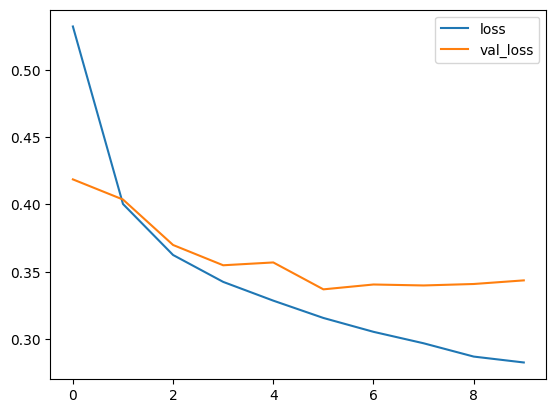
\includegraphics[width=.8\linewidth]{apendices/fig/13_IAA012_1.png}
\caption*{Fonte: O autor (2024).}
\end{figure}
\subsubsection*{Breve explicação gráfico de perda}
A linha azul 'loss' representa a função de perda no conjunto de treinamento, ou seja, o quão ruim as previsões foram nesse conjunto em relação aos valores verdadeiros. Já a linha laranja 'val\_loss' mostra a perda no conjunto de validação. A perda diminui gradualmente mostrando que a rede está convergindo para melhores resultados conforme vai sendo treinada.
\begin{lstlisting}[language=Python, style=input]
# Plotar a acurácia
plt.plot(r.history["accuracy"], label="acc")
plt.plot(r.history["val_accuracy"], label="val_acc")
plt.legend()
\end{lstlisting}
\begin{figure}[H]
\centering
\caption{Acurácia - Fashion MNIST}
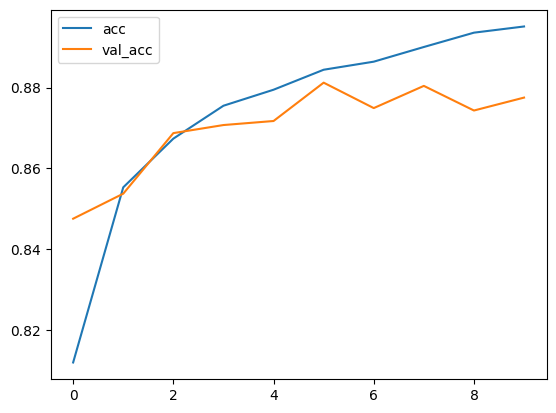
\includegraphics[width=.8\linewidth]{apendices/fig/13_IAA012_2.png}
\caption*{Fonte: O autor (2024).}
\end{figure}
\subsubsection*{Breve explicação gráfico de acurácia}
A linha azul 'acc' representa a acurácia no conjunto de treinamento, ou seja, quantas foram as previsões corretas durante o treinamento. Já a linha laranja 'val\_acc' representa a acurária no conjunto de validação, mostrando como a rede generaliza para dados que não foram utilizados no treinamento. Ambas as acurárias aumentam gradativamente indicando que a rede está aprendendo e atinge um valor mais de 87\% oque é uma boa acurácia.
\begin{lstlisting}[language=Python, style=input]
# Avaliar o modelo com a base de teste
print( model.evaluate(x_test, y_test) )
\end{lstlisting}
\begin{lstlisting}[language=, style=output]
accuracy: 0.8782 - loss: 0.3406
[0.3435542583465576, 0.8774999976158142]
\end{lstlisting}
\subsubsection*{Predições}
\begin{lstlisting}[language=Python, style=input]
y_pred = model.predict(x_test).argmax(axis=1)

# Matriz de confusão
cm = confusion_matrix(y_test, y_pred)
plot_confusion_matrix(conf_mat=cm, figsize=(7, 7),
                      show_normed=True)
\end{lstlisting}
\begin{figure}[H]
\centering
\caption{Matriz de confusão - Fashion MNIST}
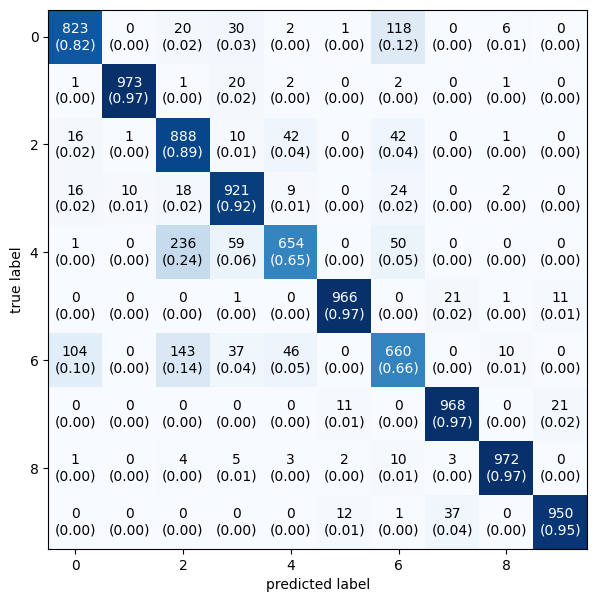
\includegraphics[width=.8\linewidth]{apendices/fig/13_IAA012_3.png}
\caption*{Fonte: O autor (2024).}
\end{figure}
\subsubsection*{Mostrar algumas classificações erradas}
\begin{lstlisting}[language=Python, style=input]
misclassified = np.where(y_pred != y_test)[0]

i = np.random.choice(misclassified)

plt.imshow(x_test[i].reshape(28, 28), cmap="gray")
plt.title("True label: %s Predicted: %s" % (y_test[i], y_pred[i]))
\end{lstlisting}
\begin{figure}[H]
\centering
\caption{Classificação errada - Fashion MNIST}
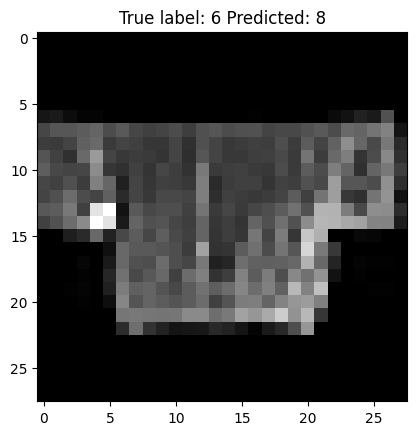
\includegraphics[width=.6\linewidth]{apendices/fig/13_IAA012_4.png}
\caption*{Fonte: O autor (2024).}
\end{figure}

%%%%%%%%%%%%%%%%%%%%%%%%%%%%%%%%%%%%%%%%%%%%%%%%%%%%%%%%%%%%%%%%%%%%%%%%%%%%%%%%%%%%%%%%%%%%%%%
\subsection*{\textbf{2 Regressão (RNA)}}
\subsubsection*{Importação das bibliotecas}
\begin{lstlisting}[language=Python, style=input]
import tensorflow as tf
import pandas as pd
import numpy as np
import matplotlib.pyplot as plt

from sklearn.model_selection import train_test_split
from sklearn.metrics import r2_score, mean_squared_error
from math import sqrt
from sklearn.preprocessing import StandardScaler, MinMaxScaler
from imblearn.over_sampling import SMOTE
from imblearn.under_sampling import RandomUnderSampler
from sklearn.utils.class_weight import compute_class_weight
from tensorflow.python.keras import backend
\end{lstlisting}
\subsubsection*{Importação dos dados}
\begin{lstlisting}[language=Python, style=input]
url = "https://archive.ics.uci.edu/ml/machine-learning-databases/wine-quality/winequality-red.csv"
data = pd.read_csv(url, delimiter=';')

data.head()
\end{lstlisting}
\begin{tcolorbox}[myoutputstyle]
\begin{table}[H]
\centering
%\caption{Dataset - Wine Quality (parte 1)}
\resizebox{\linewidth}{!}{%
\begin{tabular}{c c c c c c}
\hline
\textbf{ID} & \textbf{Fixed acidity} & \textbf{Volatile acidity} & \textbf{Citric acid} & \textbf{Residual sugar} & \textbf{Chlorides} \\
\hline
0 & 7.4 & 0.70 & 0.00 & 1.9 & 0.076 \\
1 & 7.8 & 0.88 & 0.00 & 2.6 & 0.098 \\
2 & 7.8 & 0.76 & 0.04 & 2.3 & 0.092 \\
3 & 11.2 & 0.28 & 0.56 & 1.9 & 0.075 \\
4 & 7.4 & 0.70 & 0.00 & 1.9 & 0.076 \\
\hline
\end{tabular}
}
\end{table}


\begin{table}[H]
\centering
%\caption{Dataset - Wine Quality (parte 2)}
\resizebox{\linewidth}{!}{%
\begin{tabular}{c c c c c c c c}
\hline
\textbf{ID} & \textbf{Free SO$_2$} & \textbf{Total SO$_2$} & \textbf{Density} & \textbf{pH} & \textbf{Sulphates} & \textbf{Alcohol} & \textbf{Quality} \\
\hline
0 & 11.0  & 34.0  & 0.9978 & 3.51 & 0.56 & 9.4 & 5 \\
1 & 25.0  & 67.0  & 0.9968 & 3.20 & 0.68 & 9.8 & 5 \\
2 & 15.0  & 54.0  & 0.9970 & 3.26 & 0.65 & 9.8 & 5 \\
3 & 17.0 & 60.0 & 0.9980 & 3.16 & 0.58 & 9.8 & 6 \\
4 & 11.0  & 34.0  & 0.9978 & 3.51 & 0.56 & 9.4 & 5 \\
\hline
\end{tabular}
}
\end{table}
\end{tcolorbox}
\begin{lstlisting}[language=Python, style=input]
#Dica 1. Para facilitar o trabalho, renomeie o nome das colunas para português, dessa forma:
data.columns = [
'acidez_fixa', # fixed acidity
'acidez_volatil', # volatile acidity
'acido_citrico', # citric acid
'acucar_residual', # residual sugar
'cloretos', # chlorides
'dioxido_de_enxofre_livre', # free sulfur dioxide
'dioxido_de_enxofre_total', # total sulfur dioxide
'densidade', # density
'pH', # pH
'sulfatos', # sulphates
'alcool', # alcohol
'score_qualidade_vinho' # quality
]

#Dica 2. Separe os dados (x e y) de tal forma que a última coluna (índice -1), chamada score_qualidade_vinho, seja a variável target (y)
X = data.iloc[:, :-1]  # Todas as colunas exceto a última
Y = data.iloc[:, -1].astype(float)  # Apenas a última coluna

# Verificar distribuição dos dados
data['score_qualidade_vinho'].value_counts().sort_index().plot(kind='bar')
plt.show()
\end{lstlisting}
\begin{figure}[H]
\centering
\caption{Distribuição dos dados - Wine quality}
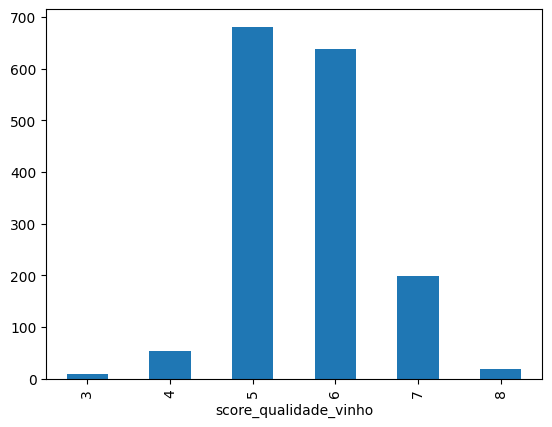
\includegraphics[width=.8\linewidth]{apendices/fig/13_IAA012_5.png}
\caption*{Fonte: O autor (2024).}
\end{figure}
\begin{lstlisting}[language=Python, style=input]
# Melhorar distribuição dos dados

#Aplicar SMOTE (oversampling) ou RandomUnderSampler (undersampling)
#Tentativa 1
smote = SMOTE(random_state=42)
#Tentativa 2
#undersampler = RandomUnderSampler(random_state=42)

#Tentativa 1
X, Y = smote.fit_resample(X, Y)
#Tentativa 2
#x_train, y_train = undersampler.fit_resample(x_train, y_train)

# Verificar a distribuição das classes após o balanceamento
print(pd.Series(Y).value_counts())
\end{lstlisting}
\begin{tcolorbox}[myoutputstyle]
score\_qualidade\_vinho\\
5.0    681\\
6.0    681\\
7.0    681\\
4.0    681\\
8.0    681\\
3.0    681\\
Name: count, dtype: int64
\end{tcolorbox}
\subsubsection*{Separação da base em treino e teste (80/20)}
\begin{lstlisting}[language=Python, style=input]
x_train, x_test, y_train, y_test = train_test_split(X, Y,
                                      test_size=0.2)
\end{lstlisting}
\subsubsection*{Pré-processamento dos dados}
\begin{lstlisting}[language=Python, style=input]
# Normalização dos dados de entrada
scaler = StandardScaler()
#scaler = MinMaxScaler()

# Ajustar o scaler aos dados de treinamento e transformar x_train
x_train = scaler.fit_transform(x_train)

# Transformar x_test
x_test = scaler.transform(x_test)
\end{lstlisting}
\subsubsection*{Criação do modelo}
\begin{lstlisting}[language=Python, style=input]
# 3 camadas
i = tf.keras.layers.Input(shape=(11,))
#x = tf.keras.layers.Dense(50, activation='relu')(i)
x = tf.keras.layers.Dense(64, activation='relu')(i)
d = tf.keras.layers.Dropout(0.2)(x)
x1 = tf.keras.layers.Dense(32, activation='relu')(d)
d1 = tf.keras.layers.Dropout(0.2)(x1)
x2 = tf.keras.layers.Dense(1)(d1)

model = tf.keras.models.Model(i, x2)
\end{lstlisting}
\subsubsection*{Compilação e treinamento do modelo}
\begin{lstlisting}[language=Python, style=input]
# Criação de funções para as métricas R2 e RMSE serem inseridas no modelo
def rmse(y_true, y_pred):
  # Converter y_true para float32 para garantir compatibilidade
  y_true = backend.cast(y_true, dtype='float32')

  return backend.sqrt(backend.mean( backend.square(y_pred - y_true), axis=-1) )

def r2(y_true, y_pred):
  # Converter y_true para float32 para garantir compatibilidade
  y_true = backend.cast(y_true, dtype='float32')

  media = backend.mean(y_true)
  num   = backend.sum (backend.square(y_true - y_pred))
  den   = backend.sum (backend.square(y_true - media))
  return (1.0 - num/den)

# Compilação
#optimizer=tf.keras.optimizers.Adam(learning_rate=0.05)
#optimizer = tf.keras.optimizers.Adam(learning_rate=0.001)
optimizer=tf.keras.optimizers.SGD(learning_rate=0.01, momentum=0.9)
#optimizer=tf.keras.optimizers.SGD(learning_rate=0.2, momentum=0.5)
#optimizer=tf.keras.optimizers.RMSprop(0.01)

model.compile(optimizer=optimizer,
              loss="mse",
              metrics=[rmse, r2])

# Early stop para epochs
early_stop = tf.keras.callbacks.EarlyStopping(
                            monitor='val_loss',
                            patience=50,
                            restore_best_weights=True)

#Treinar o modelo com ou sem pesos de classe
#r = model.fit(x_train, y_train, epochs=100, batch_size=32, validation_data=(x_test, y_test), callbacks=[early_stop])

r = model.fit(x_train, y_train, batch_size=64, epochs=150, validation_data=(x_test, y_test), callbacks=[early_stop])
\end{lstlisting}
\subsubsection*{Avaliação do modelo}
\begin{lstlisting}[language=Python, style=input]
plt.plot( r.history["loss"], label="loss" )
plt.plot( r.history["val_loss"], label="val_loss" )
plt.legend()
\end{lstlisting}
\begin{figure}[H]
\centering
\caption{Função de perda - Wine quality}
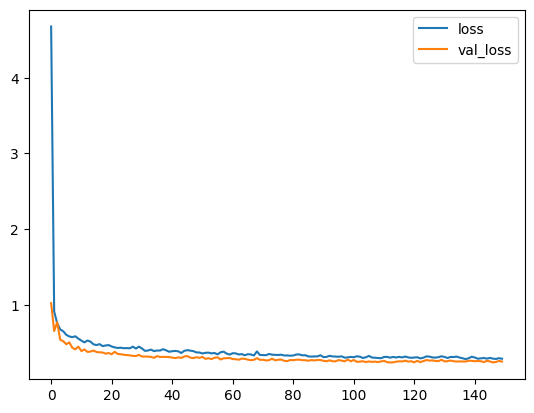
\includegraphics[width=.8\linewidth]{apendices/fig/13_IAA012_6.png}
\caption*{Fonte: O autor (2024).}
\end{figure}
\subsubsection*{Breve explicação gráfico loss}
A linha azul 'loss' representa a função de perda no conjunto de treinamento, ou seja, o quão ruim as previsões foram nesse conjunto em relação aos valores verdadeiros. Já a linha laranja 'val\_loss' mostra a perda no conjunto de validação. A rede convergiu rapidamente para um baixo valor de perda, e depois se mantém quase constante com uma mínima variação, sugerindo que talvez possa ser diminuido o número de épocas no treinamento.

\begin{lstlisting}[language=Python, style=input]
plt.plot( r.history["rmse"], label="rmse" )
plt.plot( r.history["val_rmse"], label="val_rmse" )
plt.legend()
\end{lstlisting}
\begin{figure}[H]
\centering
\caption{RMSE - Wine quality}
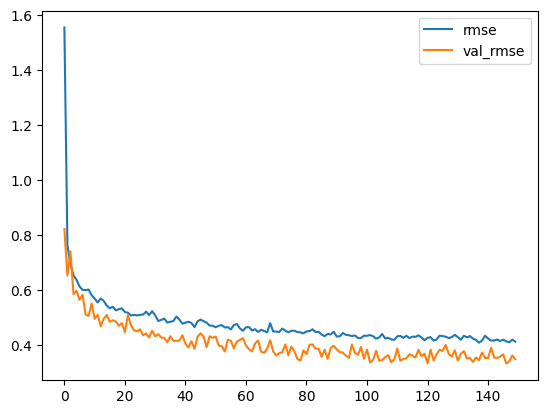
\includegraphics[width=.8\linewidth]{apendices/fig/13_IAA012_7.png}
\caption*{Fonte: O autor (2024).}
\end{figure}

\begin{lstlisting}[language=Python, style=input]
plt.plot( r.history["r2"], label="r2" )
plt.plot( r.history["val_r2"], label="val_r2" )
plt.legend()
\end{lstlisting}
\begin{figure}[H]
\centering
\caption{R2 - Wine quality}
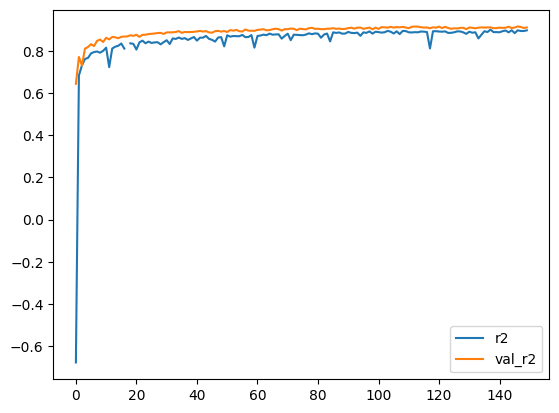
\includegraphics[width=.8\linewidth]{apendices/fig/13_IAA012_8.png}
\caption*{Fonte: O autor (2024).}
\end{figure}
\subsubsection*{Predições}
\begin{lstlisting}[language=Python, style=input]
# Predição
y_pred = model.predict(x_test).flatten()

print(y_test[:10])
print(y_pred[:10])
\end{lstlisting}
\begin{tcolorbox}[myoutputstyle]
837     7.0\\
1303    5.0\\
2092    3.0\\
3659    8.0\\
2747    4.0\\
723     5.0\\
3230    7.0\\
1164    5.0\\
808     5.0\\
3133    7.0\\
Name: score\_qualidade\_vinho, dtype: float64\\
6.3655353 6.268461  2.9856465 7.419491  4.506182  4.958458  5.962226\\
 4.9503975 5.1298738 6.320078
\end{tcolorbox}
\begin{lstlisting}[language=Python, style=input]
# Cálculo das métricas de acurácia: mse, r2 e rmse
mse  = mean_squared_error(y_test, y_pred)
rmse = sqrt(mse)
r2   = r2_score(y_test, y_pred)

# Resultados das métricas de acurácia
print("mse     = ", mse)
print("rmse    = ", rmse)
print("r2      = ", r2)
\end{lstlisting}
\begin{tcolorbox}[myoutputstyle]
mse     =  0.23897800376884185\\
rmse    =  0.4888537652190498\\
r2      =  0.9187425337397466
\end{tcolorbox}
\subsubsection*{Breve explicação das métricas de avaliação}

\begin{itemize}
    \item O MSE de $\approx0.2389$ sugere que a média dos erros quadráticos não é muito alta, o que implica que o modelo fez previsões razoavelmente boas.
    \item O RMSE de $\approx0.489$ indica que o modelo está errando pouco.
    \item Um R² de $\approx0.9187$ significa que aproximadamente 91.87\% das qualidades dos vinhos é explicada corretamente pelo modelo. Isso é um excelente desempenho para uma regressão, indicando que a RNA tem uma boa capacidade preditiva.
\end{itemize}


%%%%%%%%%%%%%%%%%%%%%%%%%%%%%%%%%%%%%%%%%%%%%%%%%%%%%%%%%%%%%%%%%%%%%%%%%%%%%%%%%%%%%%%%%%%%%%%
\subsection*{\textbf{3 Sistemas de Recomendação}}
\subsubsection*{Importação das bibliotecas}
\begin{lstlisting}[language=Python, style=input]
import tensorflow as tf
from tensorflow.keras.layers import Input, Dense, Embedding, Flatten, Concatenate, Dropout, Layer
from tensorflow.keras.models import Model
from tensorflow.keras.optimizers import SGD, Adam
from tensorflow.keras.regularizers import l2
from tensorflow.keras.callbacks import EarlyStopping

from sklearn.utils import shuffle

import numpy as np
import pandas as pd
import matplotlib.pyplot as plt
\end{lstlisting}
\subsubsection*{Importação dos dados}
\begin{lstlisting}[language=Python, style=input]
import pandas as pd

rows = []

# Abrindo o arquivo original
with open("/content/Base_livros.csv", "r") as file:
    next(file)  # Pula a primeira linha
    for line in file:
        isbn, rest = line.split(",", 1)

        rest_parts = rest.rsplit(",", 5)

        if len(rest_parts) == 6:
            titulo, autor, ano, editora, id_usuario, notas = rest_parts
            rows.append({
                "ISBN": isbn.strip(),
                "Titulo": titulo.strip(),
                "Autor": autor.strip(),
                "Ano": ano.strip(),
                "Editora": editora.strip(),
                "ID_usuario": id_usuario.strip(),
                "Notas": notas.strip()
            })

# Limpeza geral
df['ISBN'] = df['ISBN'].str.replace(r'^"|"$', '', regex=True)  # Remove aspas extras no início e fim
df['Titulo'] = df['Titulo'].str.replace(r'^""|""$', '', regex=True)  # Remove aspas ao redor do título
df['Notas'] = df['Notas'].str.replace(r';+', '', regex=True)  # Remove os ';' extras nas notas
df['Notas'] = df['Notas'].str.replace(r'^"|"$', '', regex=True)  # Remove aspas ao redor

#VERIFICAR VALORES NAN
has_nan = df.isnull().values.any()
\end{lstlisting}
\subsubsection*{Conversão de userId e movieId para categoria}
\begin{lstlisting}[language=Python, style=input]
# ID_usuario e ISBN não estão no formato certo para usar
# Embeddings > devem ser categóricos

df.ID_usuario = pd.Categorical(df.ID_usuario)
df['new_user_id'] = df.ID_usuario.cat.codes

df.ISBN = pd.Categorical(df.ISBN)
df['new_book_id'] = df.ISBN.cat.codes

#DATA AUGMENTATION

def stratified_sampling(df, n_samples=5):
    augmented_samples = []

    # Para cada usuário, pegar os livros com as diferentes notas
    for user in df['new_user_id'].unique():
        user_books = df[df['new_user_id'] == user]
        all_ratings = user_books['Notas'].unique()

        for rating in all_ratings:
            # Pegar livros com essa nota
            sampled_books = user_books[user_books['Notas'] == rating].sample(n=n_samples, replace=True)
            for _, row in sampled_books.iterrows():
                augmented_samples.append([row['new_user_id'], row['new_book_id'], row['Notas']])

    # Criar DataFrame com as interações aumentadas
    augmented_df = pd.DataFrame(augmented_samples, columns=['new_user_id', 'new_book_id', 'Notas'])
    return augmented_df

# Aplicar amostragem estratificada
augmented_df = stratified_sampling(df)
# PARA DESATIVAR DATA AUGMENTATION
#augmented_df = df

# Dimensões
N = len(set(augmented_df.new_user_id))
M = len(set(augmented_df.new_book_id))

# dimensão do embedding (tentar outros)
K = 10
\end{lstlisting}
\subsubsection*{Criar o modelo}
\begin{lstlisting}[language=Python, style=input]
# usuário
u = Input(shape=(1,))
u_emb = Embedding(N, K)(u) # saída : num_samples, 1, K
u_emb = Flatten()(u_emb)   # saída : num_samples, K

# livro
m = Input(shape=(1,))
m_emb = Embedding(M, K)(m)  # saída : num_samples, 1, K
m_emb = Flatten()(m_emb)    # saída : num_samples, K

x = Concatenate()([u_emb, m_emb])

x = Dense(1024, activation="relu")(x)
x = Dense(1)(x)

model = Model(inputs=[u, m], outputs=x)
\end{lstlisting}
\subsubsection*{Compilação do modelo}
\begin{lstlisting}[language=Python, style=input]
model.compile(
    loss="mse",
    #optimizer=SGD(learning_rate=0.08, momentum=0.9)
    optimizer=Adam(learning_rate=0.001)
)
\end{lstlisting}

\subsubsection*{Separação dos dados e pré-processamento}
\begin{lstlisting}[language=Python, style=input]
from sklearn.preprocessing import StandardScaler

#Padronização das notas, ao descomentar aqui comentar a centralização abaixo
scaler = StandardScaler()# Ajuste conforme o nome correto da coluna
augmented_df['Notas'] = scaler.fit_transform(augmented_df[['Notas']])

# Tentar converter para numérico, substituindo não numéricos por NaN
augmented_df['Notas'] = pd.to_numeric(augmented_df['Notas'], errors='coerce')

user_ids, book_ids, ratings = shuffle(augmented_df.new_user_id, augmented_df.new_book_id, augmented_df.Notas)

Ntrain = int(0.75 * len(ratings)) # separar os dados 75% x 25%

train_user = user_ids[:Ntrain]
train_book = book_ids[:Ntrain]
train_ratings = ratings[:Ntrain]

test_user = user_ids[Ntrain:]
test_book = book_ids[Ntrain:]
test_ratings = ratings[Ntrain:]

# centralizar as notas
avg_rating = train_ratings.mean()
#train_ratings = train_ratings - avg_rating
#test_ratings = test_ratings - avg_rating

linhas_na = df[df['Notas'].isnull()]
\end{lstlisting}
\subsubsection*{Treinamento do modelo}
\begin{lstlisting}[language=Python, style=input]
early_stopping = EarlyStopping(
    monitor='val_loss',
    patience=10,
    restore_best_weights=True
)

epochs = 50

r = model.fit(
    x=[train_user, train_book],
    y=train_ratings,
    epochs=epochs,
    batch_size=1024,
    verbose=2, # não imprime o progresso
    validation_data=([test_user, test_book], test_ratings),
    callbacks=[early_stopping]
)
\end{lstlisting}
\subsubsection*{Plotar a função de perda}
\begin{lstlisting}[language=Python, style=input]
plt.plot(r.history["loss"], label="loss")
plt.plot(r.history["val_loss"], label="val_loss")
plt.legend()
plt.show()
\end{lstlisting}
\begin{figure}[H]
\centering
\caption{Função de perda - Base livros}
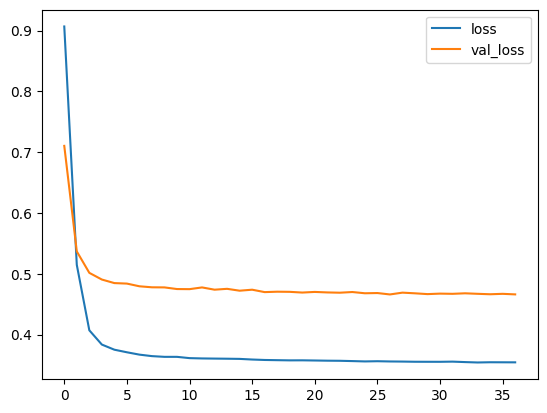
\includegraphics[width=.8\linewidth]{apendices/fig/13_IAA012_9.png}
\caption*{Fonte: O autor (2024).}
\end{figure}
\subsubsection*{Breve explicação gráfico de perda}
A linha azul 'loss' representa a função de perda no conjunto de treinamento, ou seja, o quão ruim as previsões foram nesse conjunto em relação aos valores verdadeiros. Já a linha laranja 'val\_loss' mostra a perda no conjunto de validação. O modelo começa com uma perda alta e, aparentemente, aprende rapidamente no início, o que é indicado pela queda acentuada no início da curva azul. Após um certo ponto, a curva de validação (laranja) começa a se distanciar da curva de treinamento (azul), o que pode ser um sinal de overfitting. Ou seja, o modelo está começando a se ajustar excessivamente aos dados de treinamento, mas não generaliza bem para os dados de validação, resultando em uma perda crescente no conjunto de validação.
\subsubsection*{Recomendações para o usuário 7386}
\begin{lstlisting}[language=Python, style=input]
# Gerar o array com o usuário único
# repete a quantidade de livros
input_usuario = np.repeat(a=7386, repeats=M)
book = np.array(list(set(book_ids)))

preds = model.predict( [input_usuario, book] )

# descentraliza as predições
#rat = preds.flatten() + avg_rating
# Despadroniza as predições
scaler = StandardScaler()
scaler.fit(augmented_df[['Notas']])
mean_rating = scaler.mean_
std_rating = scaler.scale_
rat = preds.flatten() * std_rating + mean_rating

# índice da maior nota
idx = np.argmax(rat)

print("Recomendação: ISBN Livro - ", book[idx], " / ", rat[idx] , "*")
\end{lstlisting}
\begin{tcolorbox}[myoutputstyle]
Recomendação: ISBN Livro -  5853  /  2.1411452293395996 *
\end{tcolorbox}
\subsubsection*{Breve explicação recomendação usuário 7386}
O modelo, para o usuário com ID 7386, recomenda o livro com ISBN e a nota associada a ele. No exemplo fornecido, a recomendação foi para o livro com ISBN 5853, e a nota prevista para o livro foi $\approx2.141$.

%%%%%%%%%%%%%%%%%%%%%%%%%%%%%%%%%%%%%%%%%%%%%%%%%%%%%%%%%%%%%%%%%%%%%%%%%%%%%%%%%%%%%%%%%%%%%%%
\subsection*{\textbf{4 Deepdream}}
Esta prática contém uma implementação mínima do DeepDream, conforme descrito neste post, do blog de Alexander Mordvintsev.

Vamos demonstrar como fazer uma rede neural "sonhar" e aprimorar os padrões surreais que ela vê em uma imagem.
\begin{figure}[H]
\centering
\caption{Prática Deepdream}
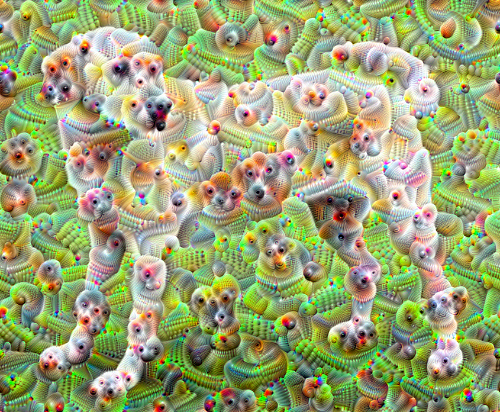
\includegraphics[width=.8\linewidth]{apendices/fig/13_IAA012_10.png}
\caption*{Fonte: O autor (2024).}
\end{figure}
\subsubsection*{Importação das bibliotecas}
\begin{lstlisting}[language=Python, style=input]
import tensorflow as tf
import numpy as np

import matplotlib as mpl

import IPython.display as display
import PIL.Image
\end{lstlisting}
\subsubsection*{Importação da imagem}
\begin{lstlisting}[language=Python, style=input]
url = "https://commons.wikimedia.org/wiki/Special:FilePath/Felis_catus-cat_on_snow.jpg"

# Download da imagem e gravação em array Numpy
def download(url, max_dim=None):
  name = url.split('/')[-1]
  image_path = tf.keras.utils.get_file(name, origin=url)
  img = PIL.Image.open(image_path)
  if max_dim:
    img.thumbnail((max_dim, max_dim))
  return np.array(img)

# Normalização da imagem
def deprocess(img):
  img = 255*(img + 1.0)/2.0
  return tf.cast(img, tf.uint8)

# Mostra a imagem
def show(img):
  display.display(PIL.Image.fromarray(np.array(img)))


# Redução do tamanho da imagem para facilitar o trabalho da RNN
original_img = download(url, max_dim=500)
show(original_img)
display.display(display.HTML('Image cc-by: <a "href=https://commons.wikimedia.org/wiki/File:Felis_catus-cat_on_snow.jpg">Von.grzanka</a>'))
\end{lstlisting}
\begin{figure}[H]
\centering
\caption{Imagem escolhida - Deepdream}
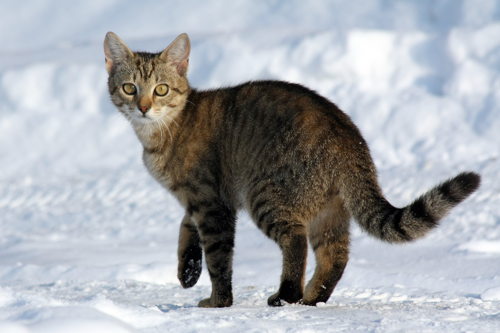
\includegraphics[width=.8\linewidth]{apendices/fig/13_IAA012_11.png}
\caption*{Fonte: O autor (2024).}
\end{figure}
\subsubsection*{Preparar o modelo de extração de recursos}
Aqui faremos o download um modelo de classificação de imagem pré-treinado. Usaremos o InceptionV3 que é semelhante ao modelo originalmente usado no DeepDream. Observe que qualquer modelo pré-treinado funcionará, embora você precise ajustar os nomes das camadas abaixo, caso deseje alterá-lo.
\begin{lstlisting}[language=Python, style=input]
base_model = tf.keras.applications.InceptionV3(include_top=False, weights='imagenet')
\end{lstlisting}

A ideia no DeepDream é escolher uma camada (ou camadas) e maximizar a "perda" de forma que a imagem cada vez mais treine as camadas.

\begin{lstlisting}[language=Python, style=input]
# Maximizando as ativações das camadas
names = ['mixed3', 'mixed5']
layers = [base_model.get_layer(name).output for name in names]

# Criação do modelo
dream_model = tf.keras.Model(inputs=base_model.input, outputs=layers)
\end{lstlisting}
\subsubsection*{Cálculo da perda (loss)}
A perda é a soma das ativações nas camadas escolhidas.

\begin{lstlisting}[language=Python, style=input]
def calc_loss(img, model):
  # Passe a imagem pelo modelo para recuperar as ativações.
  # Converte a imagem em um batch de tamanho 1.
  img_batch = tf.expand_dims(img, axis=0)
  layer_activations = model(img_batch)
  if len(layer_activations) == 1:
    layer_activations = [layer_activations]

  losses = []
  for act in layer_activations:
    loss = tf.math.reduce_mean(act)
    losses.append(loss)

  return  tf.reduce_sum(losses)
\end{lstlisting}

\subsubsection*{Subida de gradiente (Gradient ascent)}
Depois de ter calculado a perda para as camadas escolhidas, tudo o que resta é calcular os gradientes em relação à imagem e adicioná-los à imagem original.

\begin{lstlisting}[language=Python, style=input]
class DeepDream(tf.Module):
  def __init__(self, model):
    self.model = model

  @tf.function(
      input_signature=(
        tf.TensorSpec(shape=[None,None,3], dtype=tf.float32),
        tf.TensorSpec(shape=[], dtype=tf.int32),
        tf.TensorSpec(shape=[], dtype=tf.float32),)
  )
  def __call__(self, img, steps, step_size):
      print("Tracing")
      loss = tf.constant(0.0)

      for n in tf.range(steps):
        with tf.GradientTape() as tape:
          # Gradientes relativos a img
          tape.watch(img)
          loss = calc_loss(img, self.model)

        # Calculo do gradiente da perda em relação aos pixels da imagem de entrada.
        gradients = tape.gradient(loss, img)

        # Normalizacao dos gradintes
        gradients /= tf.math.reduce_std(gradients) + 1e-8

        # Na subida gradiente, a "perda" é maximizada.
        # Você pode atualizar a imagem adicionando diretamente os gradientes (porque eles têm o mesmo formato!)
        img = img + gradients*step_size
        img = tf.clip_by_value(img, -1, 1)

      return loss, img

deepdream = DeepDream(dream_model)
\end{lstlisting}
\subsubsection*{Circuito princial (Main Loop)}

\begin{lstlisting}[language=Python, style=input]
def run_deep_dream_simple(img, steps=100, step_size=0.01):

  img = tf.keras.applications.inception_v3.preprocess_input(img)
  img = tf.convert_to_tensor(img)
  step_size = tf.convert_to_tensor(step_size)
  steps_remaining = steps
  step = 0
  while steps_remaining:
    if steps_remaining>100:
      run_steps = tf.constant(100)
    else:
      run_steps = tf.constant(steps_remaining)
    steps_remaining -= run_steps
    step += run_steps

    loss, img = deepdream(img, run_steps, tf.constant(step_size))

    display.clear_output(wait=True)
    show(deprocess(img))
    print ("Step {}, loss {}".format(step, loss))


  result = deprocess(img)
  display.clear_output(wait=True)
  show(result)

  return result

dream_img = run_deep_dream_simple(img=original_img,
                                  steps=100, step_size=0.01)
\end{lstlisting}
\begin{figure}[H]
\centering
\caption{Imagem escolhida - Ciclo principal - Deepdream}
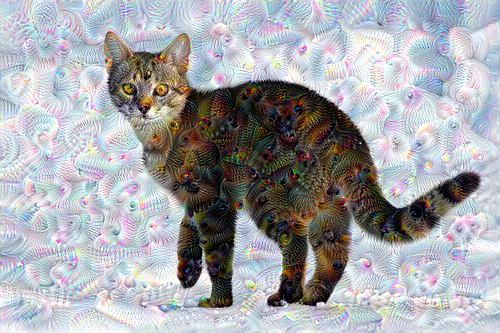
\includegraphics[width=.8\linewidth]{apendices/fig/13_IAA012_12.png}
\caption*{Fonte: O autor (2024).}
\end{figure}
Explicação: Imagem gerada durante o ciclo principal do algoritmo DeepDream, que aplica convoluções repetidas vezes para amplificar padrões reconhecidos pela rede neural, em áreas específicas da imagem, gerando texturas e formas psicodélicas, parecidas de um "sonho". Aqui ainda no Main Loop, já é observado um efeito inicial onde partes do gato mostram características "oníricas", mas ainda mantendo a estrutura básica do animal e do fundo da imagem.
\subsubsection*{Levando o modelo até um oitava}
Conseguimos gerar uma imagem. Porém, há alguns problemas com esta primeira tentativa:

\begin{enumerate}
    \item A saída é ruidosa (isso pode ser resolvido com uma perda tf.image.total\_variation).
    \item A imagem é de baixa resolução.
    \item Os padrões parecem estar acontecendo na mesma granularidade.
\end{enumerate}
\begin{lstlisting}[language=Python, style=input]
import time
start = time.time()

OCTAVE_SCALE = 1.30

img = tf.constant(np.array(original_img))
base_shape = tf.shape(img)[:-1]
float_base_shape = tf.cast(base_shape, tf.float32)

for n in range(-2, 3):
  new_shape = tf.cast(float_base_shape*(OCTAVE_SCALE**n), tf.int32)

  img = tf.image.resize(img, new_shape).numpy()

  img = run_deep_dream_simple(img=img, steps=50, step_size=0.01)

display.clear_output(wait=True)
img = tf.image.resize(img, base_shape)
img = tf.image.convert_image_dtype(img/255.0, dtype=tf.uint8)
show(img)

end = time.time()
end-start
\end{lstlisting}
\begin{figure}[H]
\centering
\caption{Imagem escolhida - Elevado oitava - Deepdream}
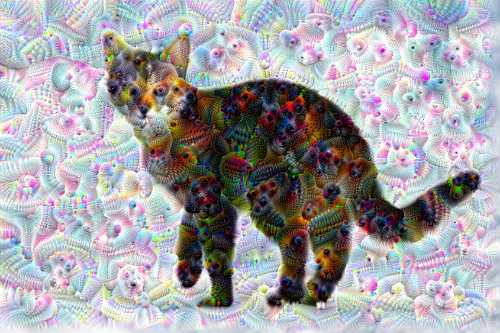
\includegraphics[width=.8\linewidth]{apendices/fig/13_IAA012_13.png}
\caption*{Fonte: O autor (2024).}
\end{figure}
Explicação: Aqui onde o modelo é elevado uma oitava a imagem gerada mostra uma intensificação maior dos detalhes oníricos. A imagem do gato começa a perder destaque para o fundo que ganha o destaque com maior preenchimento de padrões e texturas.

Elevar o modelo a uma oitava resolve os problemas de ruído, resolução, e granularidade, através da aplicação da subida de gradiente em uma escala diferente, permitindo que a imagem seja preenchida com detalhes adicionais.
\subsubsection*{Diferenças entre as imagens do Main Loop e ao elevar à oitava}
Nível de detalhe: A imagem após subir uma oitava é mais rica em detalhes, com padrões mais amplificados e complexos em comparação à imagem gerada no Main loop.

Alteração no fundo: No Main Loop, o fundo da imagem ainda mantém maior simplicidade. Após a oitava, ele é preenchido com texturas e formas oníricas adicionais.

Intensidade dos padrões: Na segunda imagem, os padrões criados pela rede neural são mais visíveis e se repetem com maior frequência em todo o corpo do gato.